\pdfbookmark{Общая характеристика работы}{characteristic}             % Закладка pdf
\section*{Общая характеристика работы}

\newcommand{\actuality}{\pdfbookmark[1]{Актуальность}{actuality}\underline{\textbf{\actualityTXT}}}
\newcommand{\progress}{\pdfbookmark[1]{Разработанность темы}{progress}\underline{\textbf{\progressTXT}}}
\newcommand{\aim}{\pdfbookmark[1]{Цели}{aim}\underline{{\textbf\aimTXT}}}
\newcommand{\tasks}{\pdfbookmark[1]{Задачи}{tasks}\underline{\textbf{\tasksTXT}}}
\newcommand{\aimtasks}{\pdfbookmark[1]{Цели и задачи}{aimtasks}\aimtasksTXT}
\newcommand{\novelty}{\pdfbookmark[1]{Научная новизна}{novelty}\underline{\textbf{\noveltyTXT}}}
\newcommand{\influence}{\pdfbookmark[1]{Практическая значимость}{influence}\underline{\textbf{\influenceTXT}}}
\newcommand{\methods}{\pdfbookmark[1]{Методология и методы исследования}{methods}\underline{\textbf{\methodsTXT}}}
\newcommand{\defpositions}{\pdfbookmark[1]{Положения, выносимые на защиту}{defpositions}\underline{\textbf{\defpositionsTXT}}}
\newcommand{\reliability}{\pdfbookmark[1]{Достоверность}{reliability}\underline{\textbf{\reliabilityTXT}}}
\newcommand{\probation}{\pdfbookmark[1]{Апробация}{probation}\underline{\textbf{\probationTXT}}}
\newcommand{\contribution}{\pdfbookmark[1]{Личный вклад}{contribution}\underline{\textbf{\contributionTXT}}}
\newcommand{\publications}{\pdfbookmark[1]{Публикации}{publications}\underline{\textbf{\publicationsTXT}}}

{\actuality}
Многие процессы и события в современном мире могут быть представлены в виде транзакционных пространственно-временных рядов. Примеры включают общение по телефону, поездки на транспорте, операции покупки/продажи, взаимодействие с социальными сетями. Каждое из этих событий представляет собой транзакцию, которая совершается в пространстве и времени. 

Развитие мобильных технологий и информационных систем привело к экспоненциальному росту объема пространственно-временных данных, что в свою очередь увеличило привлекательность исследований в этом направлении \autocite{roddick1999bibliography,cressie2015statistics,diggle2013statistical}. 

Большой интерес для урбанистики представляют собой транзакционные данные, которые описывают взаимодействие между парами или наборами объектов \cite{hawelka2014geo,paldino2015urban, ratti2010redrawing, sobolevsky2013delineating}. Транзакции могут представлять разговоры по мобильному телефону \cite{belyi2017global, kung2014exploring, amini2014impact}, операции с кредитными картами \cite{sobolevsky2016cities}, поездки на такси \cite{santi2014quantifying} и многие другие события реального мира. Транзакции помогают описать  и проанализировать социальные и экономические взаимодействия между людьми, либо между человеком и юридическим лицом.

{\progress}
Сложный формат входных данных и наличие временных, пространственных и транзакционных составляющих усложняют процесс исследования и моделирования. Даже создание простых моделей требует большого объема подготовительной работы. Существенная часть данной проблемы объясняется тем, что используемые библиотеки не предоставляют необходимые абстракции и функции для работы с пространственно-временными транзакциями.

{\aim} данной работы является разработка новых методов моделирования социального взаимодействия жителей города в пространстве и времени.

Для~достижения поставленной цели необходимо было решить следующие {\tasks}:
\begin{enumerate}[beginpenalty=10000] % https://tex.stackexchange.com/a/476052/104425
  \item Проанализировать стандартные методы моделирования взаимодействия.
  \item Разработать модель данных, которая обобщает сетевые, пространственные и временные данные внутри одной модели.
  \item Исследовать зависимость мобильности и социального взаимодействия от экономических и социальных факторов.
  \item Предложить новые методы моделирования и поиска аномалий на основе обобщенной модели пространственно-временных транзакционных данных.
\end{enumerate}


{\novelty}
\begin{enumerate}[beginpenalty=10000] 
  \item Впервые было предложено рассматривать пространственно-временные сетевые транзакции как новый класс данных.
  \item Впервые популярные методы моделирования социального взаимодействия были обобщены на случай произвольных пространственно-временных данных. 
  \item Было выполнено оригинальное исследование на тему зависимости мобильности и социального взаимодействия от экономических и социальных факторов.
\end{enumerate}


{\influence} работы состоит в разработке программной библиотеки для анализа пространственно-временных данных. Исходный код библиотеки выложен в открытый доступ, что позволяет переиспользовать реализованные методы фильтрации, агрегации и анализа любой сети. 

{\methods}
Классические методы моделирования взаимодействия в пространстве: модели гравитации и радиации.


{\reliability} полученных результатов обеспечивается предоставлением открытого исходного кода и возможностью воспроизведения полученных результатов любым заинтересованным лицом.

{\probation}
Основные результаты работы докладывались~на:
\begin{enumerate}[beginpenalty=10000]
  \item X Конгресс молодых ученых
  \item 10th International Young Scientists Conference in Computational Science (на рассмотрении)
\end{enumerate}

{\contribution} Автор играл ведущую роль в решении всех указанных задач.
 % Характеристика работы по структуре во введении и в автореферате не отличается (ГОСТ Р 7.0.11, пункты 5.3.1 и 9.2.1), потому её загружаем из одного и того же внешнего файла, предварительно задав форму выделения некоторым параметрам

%Диссертационная работа была выполнена при поддержке грантов \dots

%\underline{\textbf{Объем и структура работы.}} Диссертация состоит из~введения,
%четырех глав, заключения и~приложения. Полный объем диссертации
%\textbf{ХХХ}~страниц текста с~\textbf{ХХ}~рисунками и~5~таблицами. Список
%литературы содержит \textbf{ХХX}~наименование.

\pdfbookmark{Содержание работы}{description}                          % Закладка pdf
\section*{Содержание работы}
Во \underline{\textbf{введении}} обосновывается актуальность
исследований, проводимых в~рамках данной диссертационной работы,
приводится обзор научной литературы по~изучаемой проблеме,
формулируется цель, ставятся задачи работы, излагается научная новизна
и практическая значимость представляемой работы.


\underline{\textbf{Первая глава}} посвящена описанию обощенного представления пространственно-временных сетей, и стандартным операциям (таким как фильтрация или агрегация) для заданного представления.

Модель данных основана на ориентированном псевдографе с метками для вершин и ребер. Более формально: 
\begin{equation}
\label{eq:sttn} {
STTN = (V, A, \Sigma_V, \Sigma_A, o, d, L_V, L_A, space, time)
}
\end{equation}

V - множество вершин

А - множество дуг

$\Sigma_V$ - алфавит меток множества вершин

$\Sigma_A$ - алфавит меток множества дуг

$o: A \mapsto V$ - функция соответствия начальной вершины дуги

$d: A \mapsto V$ - функция соответствия конечной вершины дуги

$L_V: V \mapsto \Sigma_V$ - функция меток для вершин

$L_A: A \mapsto \Sigma_A$ - функция меток для дуг

$space$ - пространственная характеристика $\Sigma_V$

$time$ - временная характеристика $\Sigma_A$


Следует отметить что алфавиты $\Sigma_V$ и $\Sigma_A$ могут содержать дополнительные пространственные и временные компоненты. Функции $space, time$ отвечают за выбор пространственного и временного измерения, которое  используется моделью для пространственного/временного анализа.   

\begin{figure}[ht]
        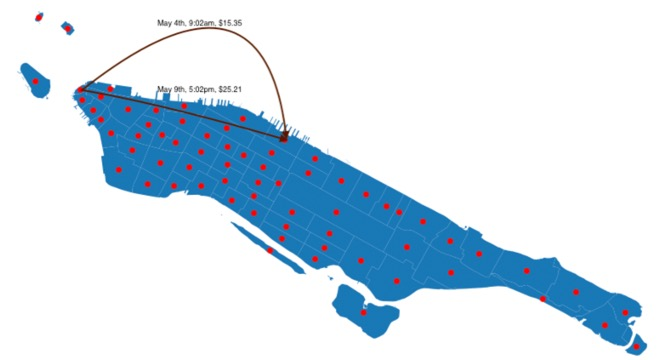
\includegraphics[width=1\linewidth]{sttn}
    \caption{Пример пространственно-временной транзакционной сети: поздки на такси.}
\end{figure}

\underline{\textbf{Вторая глава}} посвящена анализу существующих методов моделирования мобильности и социального взаимодействия. Также рассматриваются обобщения существующих моделей на случай произвольной сети (включая случаи, где доступно только временное, либо только пространственное измерение).

\underline{\textbf{Третья глава}} посвящена инновационным методам моделирования мобильности и социального взаимодействия на основе пространственных, временных и сетевых измерений. Также предлагается новый метод поиска аномалий.

\FloatBarrier
\pdfbookmark{Заключение}{conclusion}                                  % Закладка pdf
В \underline{\textbf{заключении}} приведены основные результаты работы, которые заключаются в следующем:
%% Согласно ГОСТ Р 7.0.11-2011:
%% 5.3.3 В заключении диссертации излагают итоги выполненного исследования, рекомендации, перспективы дальнейшей разработки темы.
%% 9.2.3 В заключении автореферата диссертации излагают итоги данного исследования, рекомендации и перспективы дальнейшей разработки темы.
\begin{enumerate}
  \item Предложена обобщенная модель представления для пространственно-временных транзакционных данных.
  \item Рассмотрены популярные модели взаимодействия в пространстве: модель гравитации и радиации.
  \item Предложены инновационные методы моделирования и поиска аномалий в пространственно-временных сетях.
  \item Для выполнения поставленных задач был реализована библиотека на языке программирования Python, которая позволяет применять разработанные модели для произвольного набора данных.
\end{enumerate}



\ifdefmacro{\microtypesetup}{\microtypesetup{protrusion=false}}{} % не рекомендуется применять пакет микротипографики к автоматически генерируемому списку литературы
\urlstyle{rm}                               % ссылки URL обычным шрифтом
\ifnumequal{\value{bibliosel}}{0}{% Встроенная реализация с загрузкой файла через движок bibtex8
  \renewcommand{\bibname}{\large \bibtitleauthor}
  \nocite{*}
  \insertbiblioauthor           % Подключаем Bib-базы
  %\insertbiblioexternal   % !!! bibtex не умеет работать с несколькими библиографиями !!!
}{% Реализация пакетом biblatex через движок biber
  % Цитирования.
  %  * Порядок перечисления определяет порядок в библиографии (только внутри подраздела, если `\insertbiblioauthorgrouped`).
  %  * Если не соблюдать порядок "как для \printbibliography", нумерация в `\insertbiblioauthor` будет кривой.
  %  * Если цитировать каждый источник отдельной командой --- найти некоторые ошибки будет проще.
  %
  %% authorvak
  \nocite{vakbib1}%
  \nocite{vakbib2}%
  %
  %% authorwos
  \nocite{wosbib1}%
  %
  %% authorscopus
  \nocite{scbib1}%
  %
  %% authorpathent
  \nocite{patbib1}%
  %
  %% authorprogram
  \nocite{progbib1}%
  %
  %% authorconf
  \nocite{confbib1}%
  \nocite{confbib2}%
  %
  %% authorother
  \nocite{bib1}%
  \nocite{bib2}%

  \ifnumgreater{\value{usefootcite}}{0}{
    \begin{refcontext}[labelprefix={}]
      \ifnum \value{bibgrouped}>0
        \insertbiblioauthorgrouped    % Вывод всех работ автора, сгруппированных по источникам
      \else
        \insertbiblioauthor      % Вывод всех работ автора
      \fi
    \end{refcontext}
  }{
  \ifnum \totvalue{citeexternal}>0
    \begin{refcontext}[labelprefix=A]
      \ifnum \value{bibgrouped}>0
        \insertbiblioauthorgrouped    % Вывод всех работ автора, сгруппированных по источникам
      \else
        \insertbiblioauthor      % Вывод всех работ автора
      \fi
    \end{refcontext}
  \else
    \ifnum \value{bibgrouped}>0
      \insertbiblioauthorgrouped    % Вывод всех работ автора, сгруппированных по источникам
    \else
      \insertbiblioauthor      % Вывод всех работ автора
    \fi
  \fi
  %  \insertbiblioauthorimportant  % Вывод наиболее значимых работ автора (определяется в файле characteristic во второй section)
  \begin{refcontext}[labelprefix={}]
      \insertbiblioexternal            % Вывод списка литературы, на которую ссылались в тексте автореферата
  \end{refcontext}
  % Невидимый библиографический список для подсчёта количества внешних публикаций
  % Используется, чтобы убрать приставку "А" у работ автора, если в автореферате нет
  % цитирований внешних источников.
  \printbibliography[heading=nobibheading, section=0, env=countexternal, keyword=biblioexternal, resetnumbers=true]%
  }
}
\ifdefmacro{\microtypesetup}{\microtypesetup{protrusion=true}}{}
\urlstyle{tt}                               % возвращаем установки шрифта ссылок URL
